\chapter{Java Enterprise Prototyp}
\label{jee_proto}
\def \currentAuthor{Jakob Tomasi}
Aufgrund der bereits geschilderten Nicht-Durchführbarkeit einer Adaption von \getOst\ wurde ein Prototyp für ein Ticketsystem entworfen, welcher die vom Landesschulrat und den Tiroler Schulen benötigten Funktionen mitbringt. Die Anforderungen für dieses System sind im Grunde die gleichen, welche zu Beginn an die \getOst-Adaption gestellt wurden.
\paragraph{}
Ein Auszug dieser Anforderungen sind:

\begin{itemize}
	\item Usability: Das System soll ohne lange Schulungsphasen oder Einlernzeit verwendet werden können. Unter Verwendung ist hauptsächlich das Absetzten von Supporttickets definiert.
	\item Mobility: Das Web-Frontend soll auch auf Smartphones und Tablets verwendet werden können und die gleichen Funktionen wie auf dem PC liefern.
	\item Adaptability: Sollten sich Anforderungen, Best Practices oder Sicherheitsanforderungen ändern, sollen diese mit so geringem Aufwand als möglich implementiert werden können.
\end{itemize}

Dieser Prototyp wurde mit der Absicht erstellt, die Durchführbarkeit bzw. Machbarkeit eines Ticketsystems entsprechend den Anforderungen des Landesschulrates und insbesondere Herrn \getHammerl\ zu entsprechen. Damit wird also geklärt, dass Java Enterprise Edition als Basistechnologie für ein solches System eingesetzt werden kann. Damit besteht eine Grundlage, an der kommende Projekte anknüpfen können.

\section{Technologie}
Für den Prototyp des Ticketsystems wurde Java Enterprise Edition ausgesucht. Diese Entscheidung basiert auf der Absicht, die bei \getOst\ gezogenen Schlüsse zu beachten und die Probleme die bei \getOst\ auftraten zu vermeiden.
\paragraph{}
JavaEE erscheint hierfür besonders geeignet, da es (in dem Verwendungsmodus, der an der Schule gelehrt wurde) von sich aus das MVC-Entwurfsmuster anwendet (mehr im nächsten Abschnitt).
\paragraph{}
Des Weiteren eignet sich JavaEE für die Beseitigung der Schwächen \getOst s durch die relativ strengen Sprachkonventionen und die (beinahe) unausweichliche Objektorientierung.

\section{Architektur}
Als Basis für die Systemarchitektur wird das Model View Controller Muster verwendet. Das bedeutet die Trennung zwischen JavaBeans (Model), die direkt mit der Persistenzebene (Datenbank) arbeitet, der Benutzerschnittstelle (View; Webschicht) und der Logik (Controller; Anwendungsschicht).

Das Lehrbuch fasst das Entwurfsmuster wie folgt zusammen und bringt dessen Sinn sowie Existenzberechtigung im Evaluationsprogramm \glqq Ticketsystem\grqq\ auf den Punkt:

\blockcquote{javaeeworkshop}{
	Das MVC ist ein Muster, das vorgibt, wie Darstellung, Logik und Daten in einer Applikation getrennt werden sollen. Ziel dieser Trennung ist die Verbesserung der Programmstruktur und damit die Wartbarkeit, Erweiterbarkeit, und Wiederverwendbarkeit des Codes.
	Das Modell kapselt die Daten und enthält je nach MVC-Ausprägung ggf. auch die fachliche Logik. Die View visualisiert das Modell und der Controller realisiert die Anwendungssteuerung Der Controller reagiert auf Benutzerinteraktionen innerhalb der View und aktualisiert ggf. die Daten am Modell. Die View wiederum passt sich je nach Ausprägung des MVC entweder automatisch an das veränderte Modell an oder wird durch den Controller über die Ausprägung informiert.
}

\paragraph{CRUD} Funktionalität vereint die folgenden Persistenzfunktionen:\\
\textbf{C}reate, \textbf{R}ead, \textbf{U}pdate, \textbf{D}elete

Damit ist also die Möglichkeit gemeint, auf die Persistenzschicht der Anwendung modifizierend zuzugreifen. Hierfür wird die Java Persistence API 2.0 (JPA) verwendet. Führt ein User also eine Operation über die Java Server Faces aus (mehr dazu unter \ref{jsf}), wird dies über die Enterprise JavaBeans an die JPA weitergereicht.

\section{Benutzerschnittstellen}
\label{jsf}
Benutzerschnittstellen werden in Java Enterprise Edition - Anwendungen mit der Technologie \glqq Java Server Faces \grqq umgesetzt. Früher wurde \glqq Java Server Pages \grqq verwendet, weiches 1999 erschien und mittlerweile veraltet ist. Java Server Faces ist ein Framework für Oberflächen von Webanwendungen. Folgende Teilkomponenten werden grundsätzlich für JSF benötigt:

\begin{itemize}
	\item Java Development Kit wurde installiert und eingebunden
	\item Servlet-Container (bspw. Apache Tomcat) ist einsatzbereit
\end{itemize}
\paragraph{}
In der Abbildung \ref{Abb_Jsf_XHTML_Code} befindet sich beispielhaft ein Auszug aus der XHTML-Datei ListTickets.xhtml. Sie oberflächlich gesehen dafür zuständig, eine Tabelle von Tickets und deren detaillierten Eigenschaften anzuzeigen. Des Weiteren finden Sich auch Navigationselemente in der Datei. Solche Tags tragen die Bezeichnung \glqq commandLink\grqq. Definiert in ihrer \glqq action \grqq -Eigenschaft befindet sich ein Expression-Language (EL) Ausdruck welcher auf eine Methode der TicketController Klasse verweist. Ausdrücke der EL sind immer umschlossen von geschweiften Klammern und geführt von einer Raute: \#\{Klassenname.Datenfeld\}, als kleines Beispiel.
\paragraph{}
Eine weitere Komponente die hervorzuheben ist, ist der DataTable. Diese Komponente stemmt die Hauptaufgabe der Seite. Sie bezieht eine Liste von Tickets mit dem EL-Ausdruck \glqq \#\{tplTicketController.items\}\grqq; eine Laufvariable \glqq item\grqq hält also ein Ticket. Die Laufvariable durchläuft jedes Ticket genau ein mal, vergleichbar mit einer klassischen For-Schleife. So werden die Eigenschaften jedes Tickets in einer Zeile des DataTable dargestellt.

\begin{figure}[h]
	\centering
	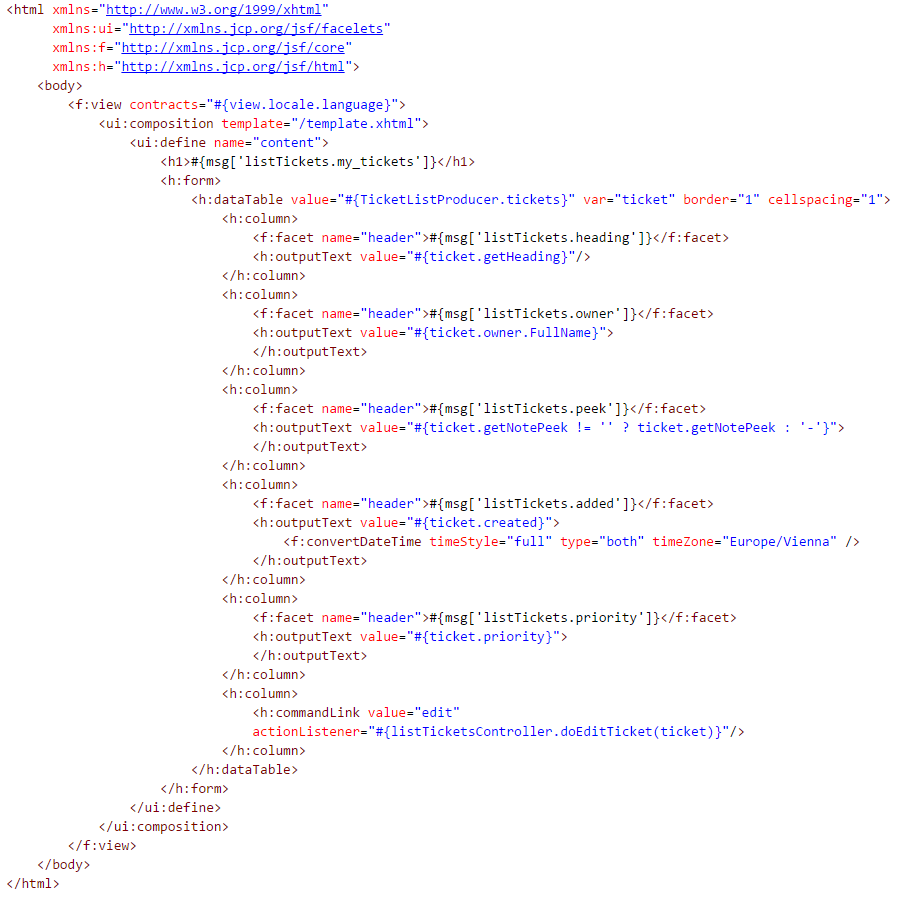
\includegraphics[scale=0.75]{figures/serverFacesCode.png}
	\caption{Ausschnitt JSF XHTML Datei}
	\label{Abb_Jsf_XHTML_Code}
\end{figure}

\newpage
\section{Klassenentwurf}

\begin{figure}[h]
	\centering
	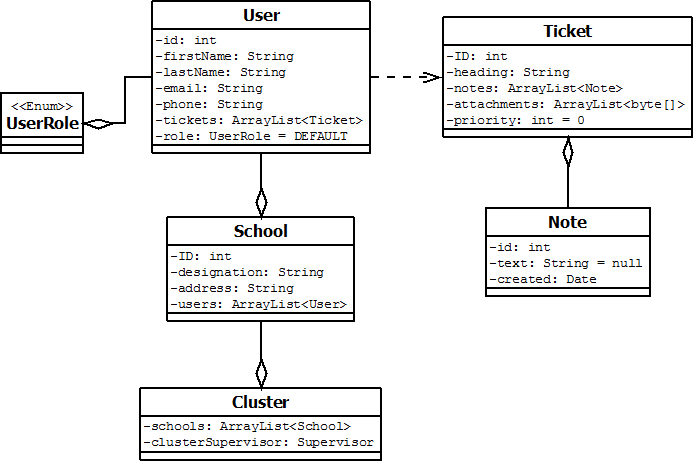
\includegraphics[scale=0.6]{figures/klassenentwurf_java_ticketsys_export.png}
	\caption{Klassenentwurf Java EE Ticketsystem}
	\label{Abb_Klassendesign_TicketSys}
\end{figure}

In Abbildung \ref{Abb_Klassendesign_TicketSys} ist ein simpler Entwurf der Model-Klassen des Ticketsystems als Klassendiagramm dargestellt. Der Benutzer (User) hält Informationen wie deren Namen, Kontaktdetails und eine Liste der vom User erstellten Tickets für die folgenden Rollen:

\begin{description}
	\item[IT Manager bzw. Managerinnen (Managers):] Eine Person an Tirols Schulen, verantwortlich für die lokale Infrastrukturbetreuung und Fehlerreporting
	\item[Systembetreuer bzw. Systembetreuerinnen (Supervisors):] Bearbeitet Meldungen (Tickets) für einen Schulcluster
	\item[Administratoren/Administratorinnen:] Eine Person des Landesschulrates, verantwortlich für das Gesamtsystem (\getHammerl).
\end{description}

Damit steht die Klasse User im Zentrum des Systems. Die Ticket-Klasse (oder eine Entität des Typs Ticket) hat eine Überschrift, eine Priorität, welche vom User (meist IT Manager(in)) definiert wird, eine Liste an Notes (Fehlerbeschreibungen, Nachrichten in Blogpost-Form) und eine Menge an Dateianhängen.